
\section{Solution}
\label{sec:solution}

\subsection{Understanding the Problem}
In order to provide a solution to a problem, that problem must first be well-defined. At a high level, this problem can be defined as needing to determine how `active' the MSC is at a given time. How does one define `active,' though? What does it mean for the MSC to be `busy' or not?

An obvious method for determining the activity is to count the number of people in the MSC. Too many people is, after all, the problem being addressed in this project. There are also more indirect measurements of activity in the center. These include sound level, whether or not there is motion, and how many lights are on in the room.

The combination of these factors can help paint a picture of how busy the MSC is at a given time. So, this project provides insight into the problem by collecting data on these factors over the course of a week, with the hope that any patterns in MSC activity will be revealed.

\subsection{Collecting Data}
This project needed to unobtrusively collect the previously mentioned information for a week. This was accomplished with a Raspberry Pi 3. The Raspberry Pi is small enough to be easily disguised for concealed data collection and has the necessary GPIO connections for compatibility with requisite sensors. Using Python, the data can then be processed and aggregated as shown in Figure \ref{fig:flowchart}. Data was collected between $5/1/18$ and $5/8/18$.

\subsubsection{Sensors}
As previously mentioned, there are four features that the Pi needed collect data on: sound, light, motion, and number of people. Sound and light data are both collected using the respective Grove sensors from Seeed.\footnote{\url{https://www.seeedstudio.com}} These sensors connect to the Pi through a GrovePi+ (see Figure \ref{fig:breadboard}). Motion and people data both originate from camera input. A Pi Camera is connected to the Raspberry Pi through the dedicated port.

\begin{figure}[t]
    \centering
    \includegraphics[width=0.97\linewidth]{figs/listening-station_bb.png}
    \caption{Diagram of listening station components. Sensors are Grove sound sensor (top) and Grove light sensor (bottom). Pi Camera is not shown.}
    \label{fig:breadboard}
\end{figure}

\subsubsection{Processing Camera Data}
The Pi Camera provides a video feed of the MSC, however that feed needs to be transformed into the desired features (i.e. whether or not there is motion, the number of people in the room). This is accomplished with OpenCV (Open Source Computer Vision Library) \cite{opencv}. This library is aimed at real-time computer vision, making this project a perfect application.

There are two components to the OpenCV processing used in this project, and they both implement motion detection \cite{motion}. First, OpenCV simply analyzes the video to determine whether or not there is motion in the frame at a given point (i.e. when data is collected). It does this by keeping track of an average `background frame.' This background frame represents the parts of the frame that never move. Then, every new frame is compared to the background frame, and if there is any difference between the two, the program determines that there is motion in the frame. Differences are only recognized if greater than a predefined threshold, $\theta$, so that noise in the image is ignored.

Finally, the Pi must be able to count the number of people in the room. This process happens in simultaneity with the previously discussed motion detection. When difference detection is executed on every frame, it does so such that any differences are grouped into \textit{contours}.

If a frame is a graph $F$ where each pixel is a vertex, a \textit{contour} is a spanning tree $T$ of a subgraph $G$ of $F$ such that
\begin{gather}
    \forall v \in V(T) : \Delta v > \theta
\end{gather}
and
\begin{gather}
    \text{min} \leq \left | V(T) \right | \leq \text{max}
\end{gather}
where \textit{min} and \textit{max} are predefined values. This definition proves useful, as is allows large clusters of changing pixels to be interpreted as single `objects.' Given that, by and large, humans are the only moving objects in the MSC, this effectively becomes a method for tracking people in the room.

There are a few key problems with this method, though. How is the computer to know whether or not a contour is a person? As previously mentioned, humans are generally the only things that will be moving in the frame, however this cannot be guaranteed. A person's head and arm could be accidentally counted as individual objects or a small change in the background could trigger a contour. The parameters $\theta$, \textit{min}, and \textit{max} are intended to address these problems. By setting proper values for these parameters (see Figure \ref{fig:params}), the program will only track contours with a specific area and only if there is a significant enough difference from the background. While this method is still hardly perfect, it is certainly better than any feasible alternative.\footnote{The next best alternative would be single-frame object detection via haarcascades. However, there is too much uncertainty in the arrangement of the subjects for this method to be viable.}

\begin{figure}[t]
    \centering
    \begin{tabular}{c|c|c|c|c}
    \hline 
    \hline
        \textbf{Min} & \textbf{Max} & $\theta$ & \textbf{Resolution} & \textbf{FPS}  \\
        \hline 
        1500 & 40000 & 2 & $1296 \times 730$ & 16 \\
        \hline 
        \hline
    \end{tabular}
    \caption{Values of data collection parameters. $\theta$ is the threshold for difference detection.}
    \label{fig:params}
\end{figure}

\subsubsection{Data Aggregation and Storage}
In order to discover trends in the data over time, data is collected at regular intervals. At the beginning of every 24-hour period, a new \texttt{DataFrame} \cite{mckinney2014pandas} is created to hold the data for that interval. Then, at the beginning of every minute, the following features are captured as the given datatypes:
\begin{itemize}
    \item Timestamp: \texttt{datetime} object
    \item Light: \texttt{int}, higher value means more light
    \item Sound: \texttt{int}, higher value means louder sound
    \item Motion: \texttt{bool}
    \item Contour Average: \texttt{float}, the average number of contours per frame for the given minute
    \item Image Name: \texttt{str}
\end{itemize}
This data is then appended to the current \texttt{DataFrame} as an entry. The video frame that was analyzed is then saved as an image with bounding boxes drawn around all contours that were found in the frame (the `Image Name' feature refers to this image's filename).

After 1440 entries have been collected (one days worth), the current \texttt{DataFrame} is saved to a CSV file, then freed from memory. The entire process then repeats. This is done to reduce the memory requirements of the program and to ensure data is saved reasonably frequently.

\begin{figure}[h]
    \centering
    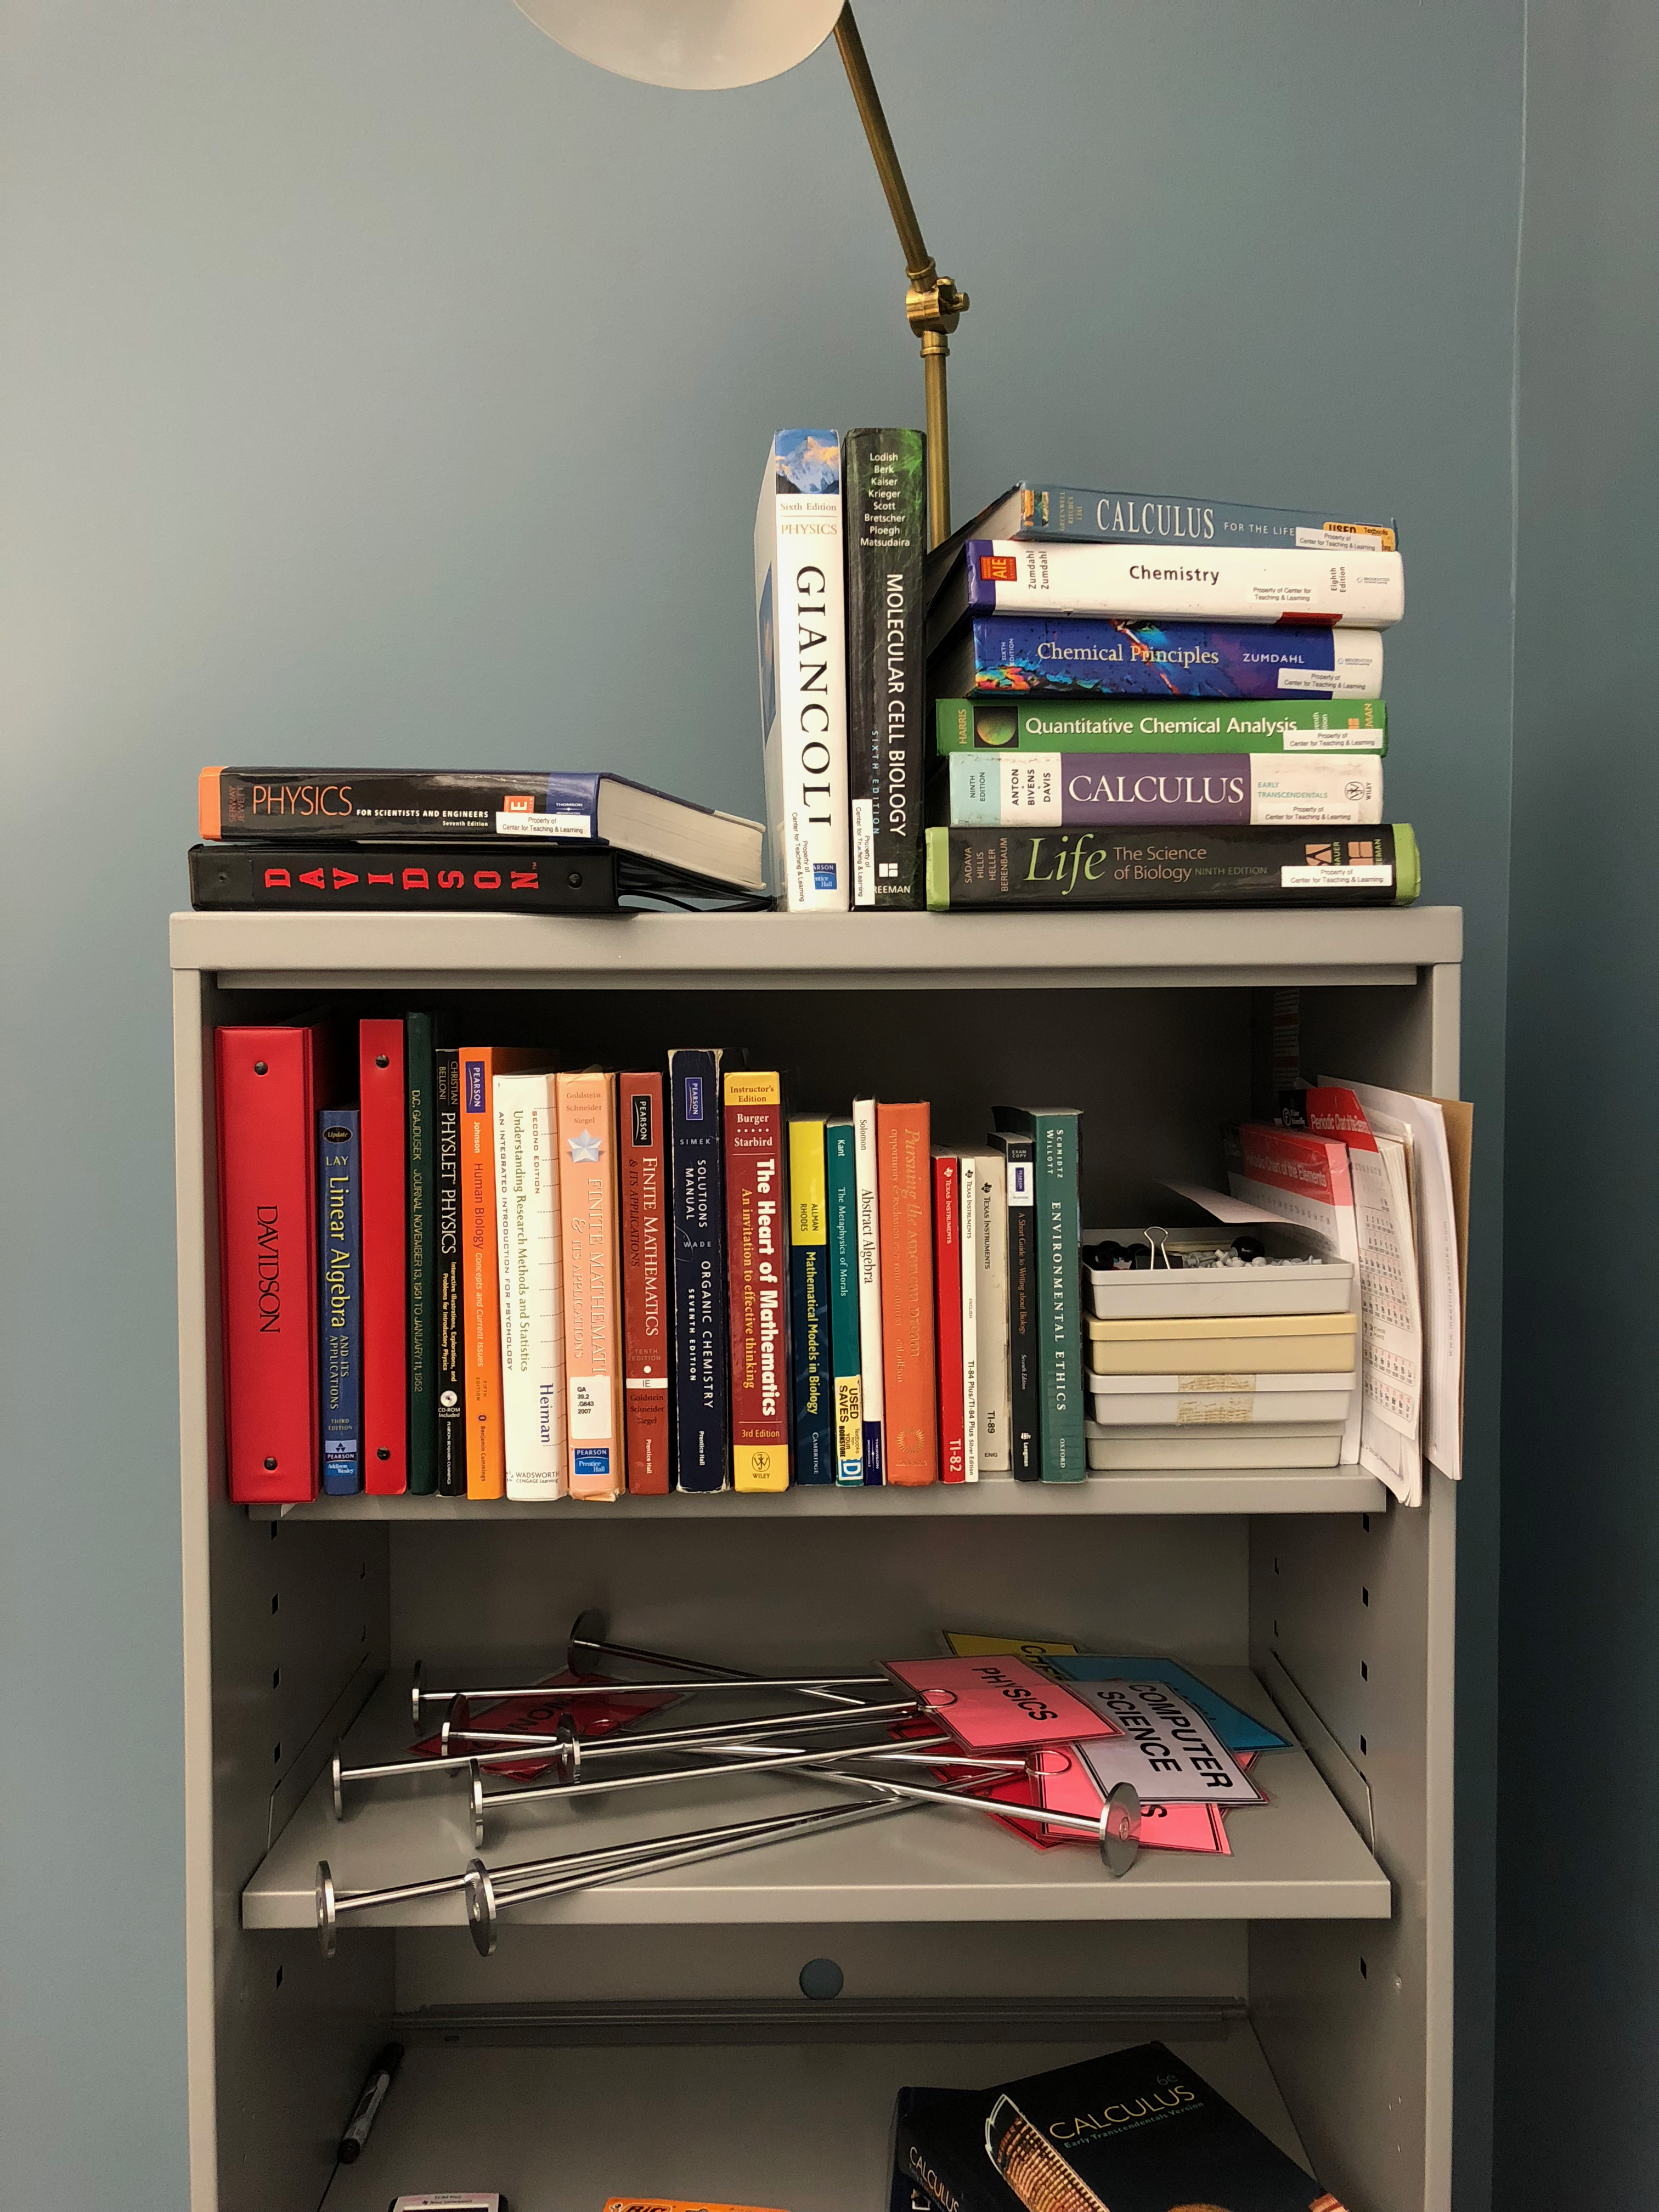
\includegraphics[width=0.97\linewidth]{figs/IMG_0627.jpg}
    \caption{Raspberry Pi as positioned during data collection (black and red `Davidson' binder on top-left of the bookshelf).}
    \label{fig:disguised}
\end{figure}

\begin{figure}[h]
    \centering
    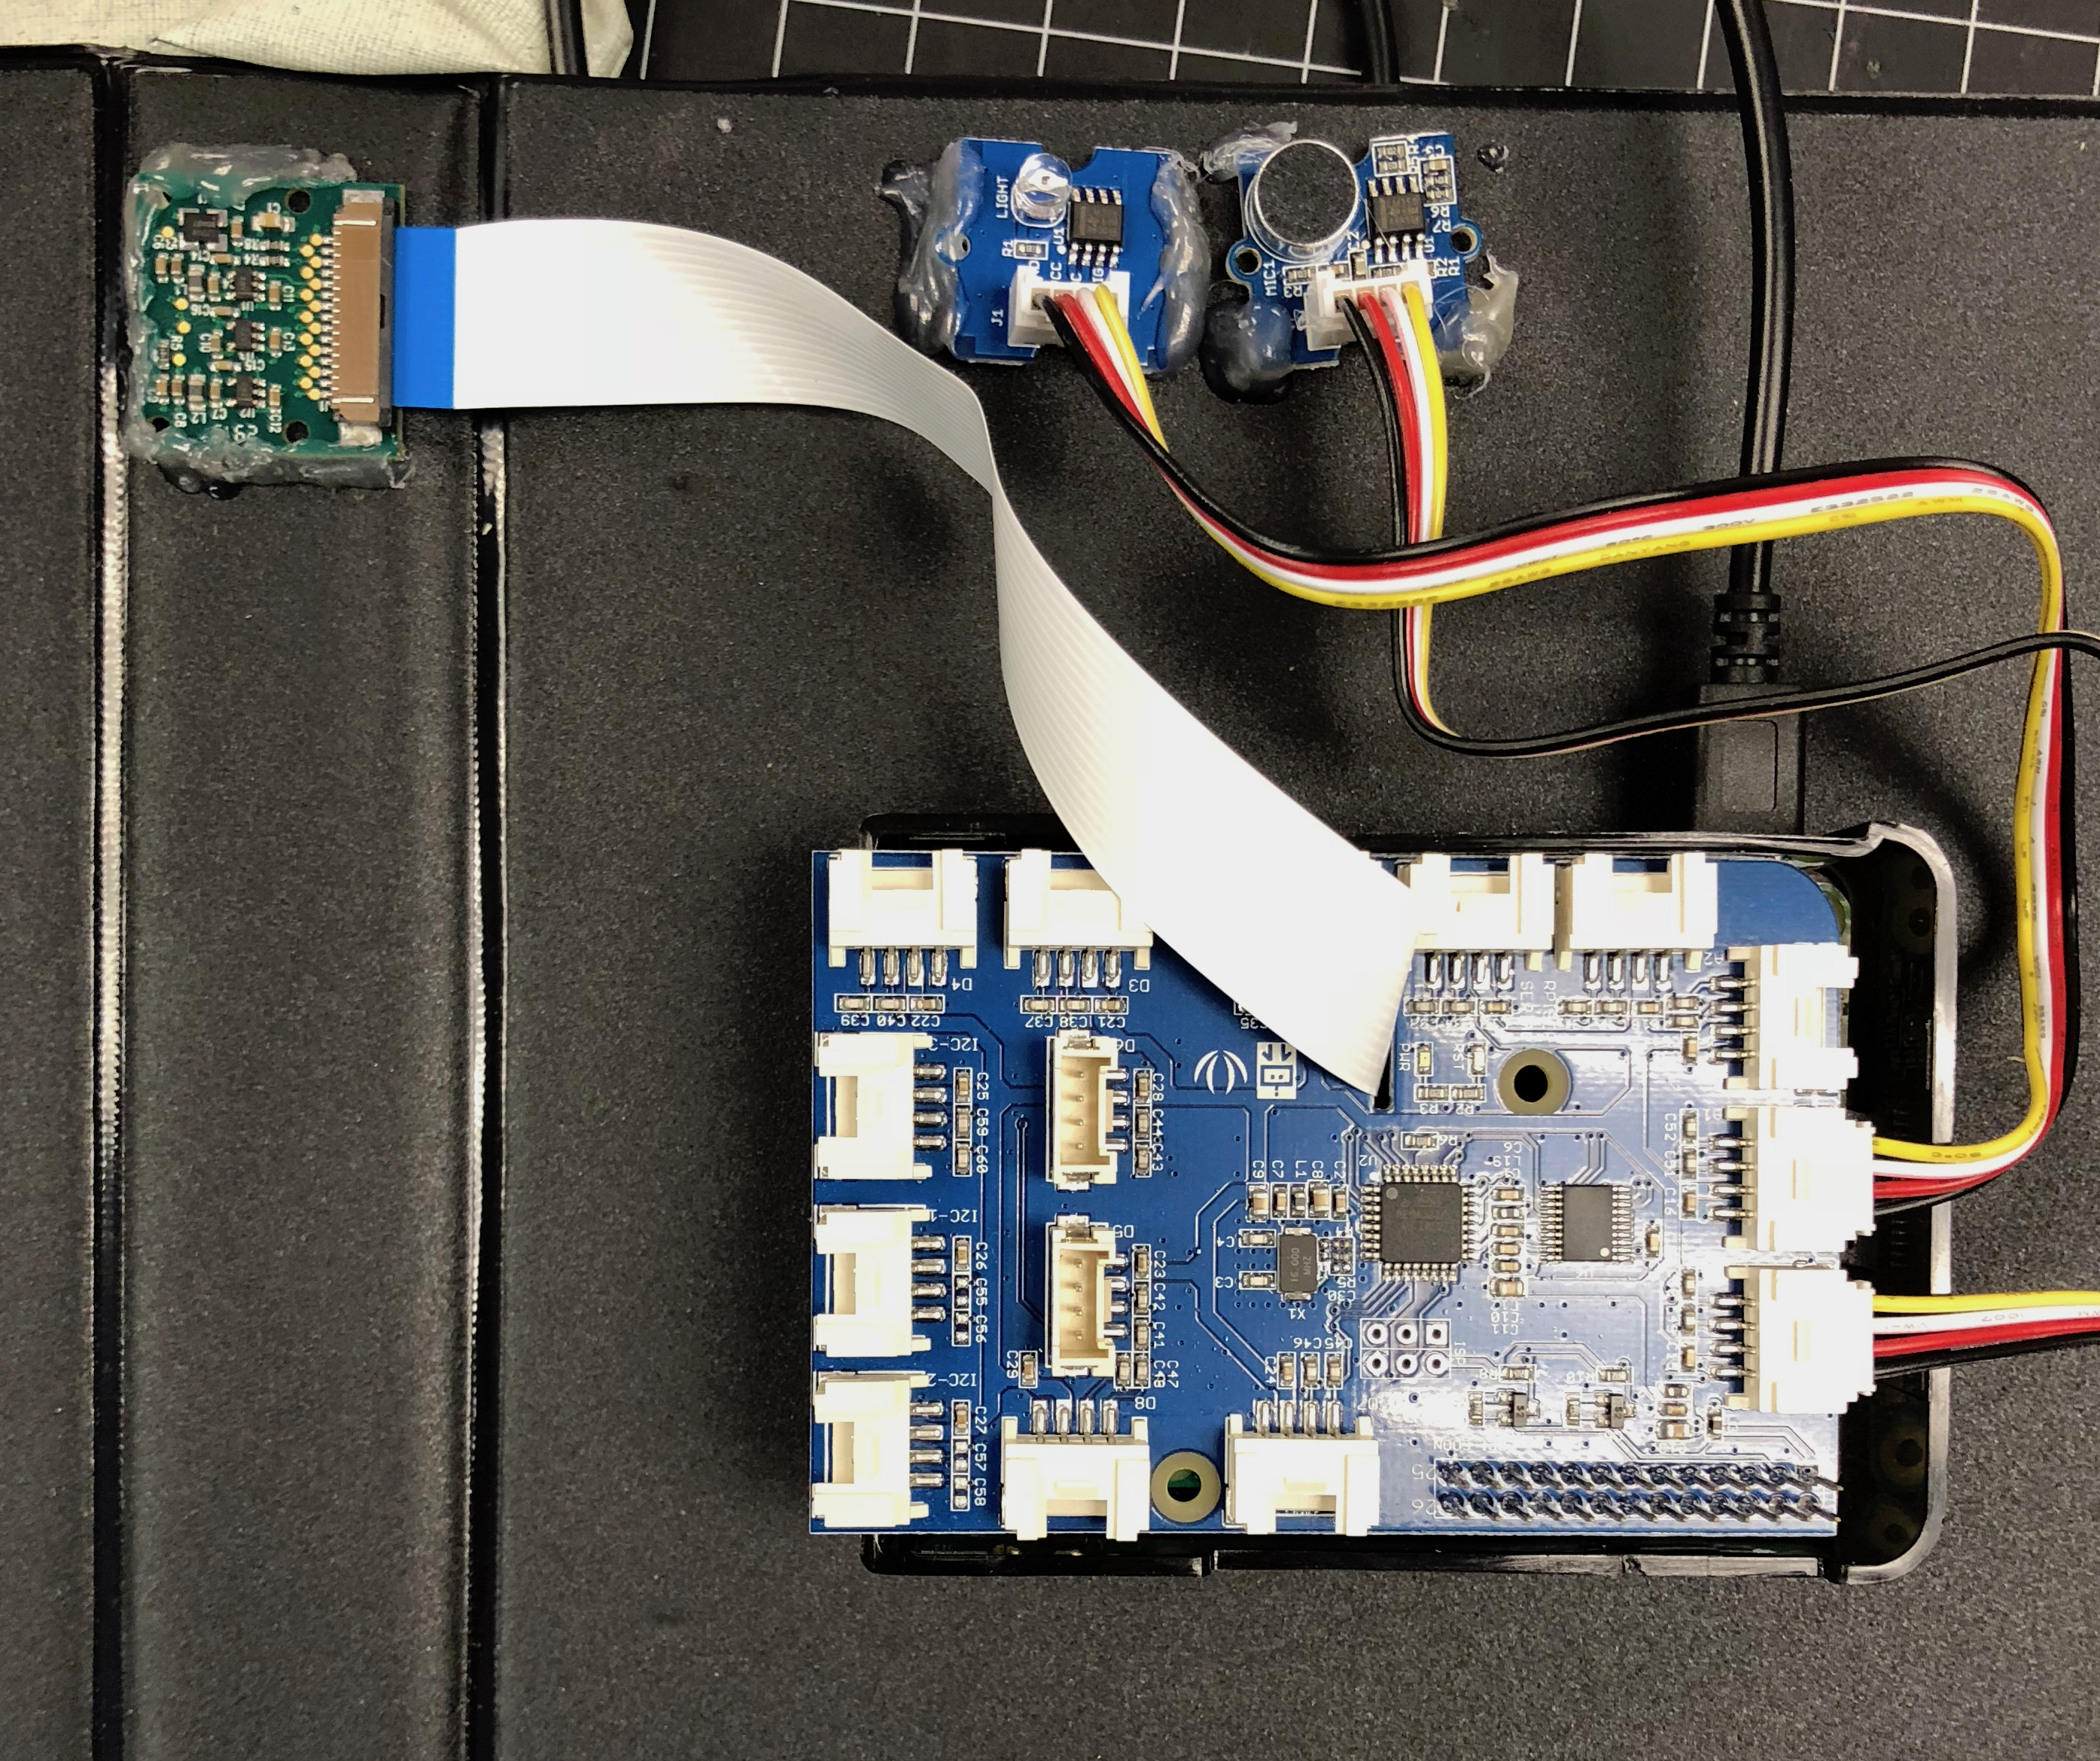
\includegraphics[width=0.97\linewidth]{figs/IMG_0621.jpg}\\
    \vspace{2mm}
    \includegraphics[width=0.97\linewidth]{figs/IMG_0622.jpg}
    \caption{Two views of the binder disguise. Top image shows Raspberry Pi and sensors positioned inside the binder. Bottom image shows where camera is hidden.}
    \label{fig:binder}
\end{figure}

\subsection{Collection Device Disguise}
In order to disguise the Raspberry Pi and sensors into the environment, they are enclosed within a three-ring binder. During the data collection period, the binder sat on top of a bookshelf in the MSC, which effectively camouflaged the device (see Figure \ref{fig:disguised}).

The Raspberry Pi, light sensor, and sound sensor are simply glued to the inside of the binder so that they are concealed. The Pi Camera rests in a small hole in the spine of the binder so that it can `see' the room (see Figure \ref{fig:binder}). Power is provided via an extension cord that runs down the back of the bookshelf.


